\paragraph{}
        A partir de nos recherches sur le domaine et les algorithmes existants pour la réalisation de notre cahier des charges, nous avons rédigé un cahier des charges pour définir les besoins fonctionnels et non fonctionnels de notre projet. Ca cahier est un contrat passé entre les clients et les programmeurs, qui définit de façon exhaustive les engagements de ces derniers vis à vis du produit final.

\paragraph{}
        Pour un tel logiciel, les besoins fonctionnels sont relativement simples à cerner, à savoir la création d'une scène, sa manipulation, et les prises de vue pour obtenir les rendus demandés dans le sujet. 
        Toutefois, les besoins non fonctionnels, même s'ils peuvent être clairement énoncés par le client, sont bien souvent implicites et doivent être déterminés en fonction du discours tenu. Pour un logiciel de synthèse d'images, la fluidité d'affichage est bien souvent un besoin essentiel, car l'utilisateur s'attend à une certaine rapidité du logiciel lors de la manipulation de la scène et de la génération de rendus. 
        Mais d'autres besoins, à savoir la portabilité du logiciel et sa maintenabilité, ont également été exprimés par les clients et ont été considérés comme essentiels pour ce projet. En effet, l'utilisaton de ce logiciel, au moins sous les systèmes d'exploitation Linux et Windows, était importante pour pouvoir travailler sur différentes machines dans leur travail. 
        De plus, un tel logiciel pouvait être amené à être amélioré ou réutilisé en partie dans de futurs projets, et c'est pourquoi il devait être facilement maintenable.

\paragraph{}
        Ces besoins ont apportés des contraintes quand à la réalisation du logiciel, par exemples sur les langages et les bibliothèques utilisées.
            Pour s'assurer de la faisabilité des besoins fonctionnels et non fonction    nels du projet, deux prototypes ont été mis en place : un prototype de fichier XML pour réfléchir au format de sauvegarde et de chargement de la scène, et un prototype de scène en trois dimensions pour tester les fonctionnalités possibles avec le langage C++ et les bibliothèques que nous souhaitions utiliser : Qt et OpenGL pour Qt. Ce prototype aura également permis de s'assurer de la portabilité de ces bibliothèques, ainsi que de la fluidité potentielle du futur logiciel.

            Le prototype XML aura permis de réfléchir aux informations importantes à stocker pour pouvoir recréer une scène à l'identique. Tout d'abord, les informations relatives aux objets doivent être stockées, telles que leur nom et leur fichier d'origine, mais également leur position, leur orientation et leur échelle. Les informations relatives à la caméra sont également essentielles pour retrouver l'angle d'observation de la scène, et les informations à stocker sont sa position, son orientation, ou encore son angle de vue. Le prototype d'origine du fichier XML est donné dans la partie Annexe du Cahier des Charges, lui-même présent en Annexe de ce rapport. Un exemple de fichier XML obtenu à partir de ce prototype est également donné en Annexe.

            Le prototype logiciel réalisé en C++ a permis de mettre en place une première version de scène contenant un objet obtenu grâce à une première version de parseur de fichiers d'extension PLY. La manipulation de cette scène a permis de tester quelques valeurs de fluidité pour pouvoir se rendre compter des capacités d'affichage des bibliothèques utilisées, qui semblaient satisfaire nos attentes. De plus, le test du prototype sur des machines Windows et Linux ont montré la portabilité des bibliothèques, même si les versions de shaders utilisées auront posé problème par la suite comme il est détaillé dans la partie suivante de ce rapport. Un exemple d'affichage du prototype initial est donné dans la [FIGURE N°], et des exemples de l'affichage final seront donnés plus tard dans ce rapport.

\paragraph{}
        Pour satisfaire le besoin d'extensibilité de notre projet, nous avons mis en place une architecture modulaire pour permettre à notre logiciel d'être modifié de façon simple. L'architecture principale est donné dans la \ref{fig:archi}.

\begin{figure}[h]
	\centering      
	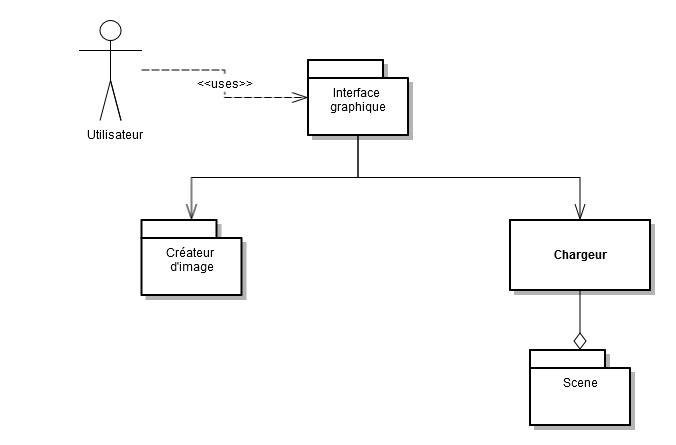
\includegraphics[scale=0.5]{diag_packages.jpg}
	\caption{\label{fig:archi} Diagramme des paquetages, architecture globale de la scène \protect \footnotemark }
\end{figure}
\footnotetext{Réalisé grâce au logiciel Gliffy : \url{www.gliffy.com}}

        Les besoins en modularité de notre projet se reflète particulièrement dans le paquetage Création de l'architecture, qui permet la création des différents rendus que le logiciel permet d'obtenir. L'architecture de ce paquetage est donné dans la \ref{fig:creation}.

\begin{figure}[h]
	\centering      
	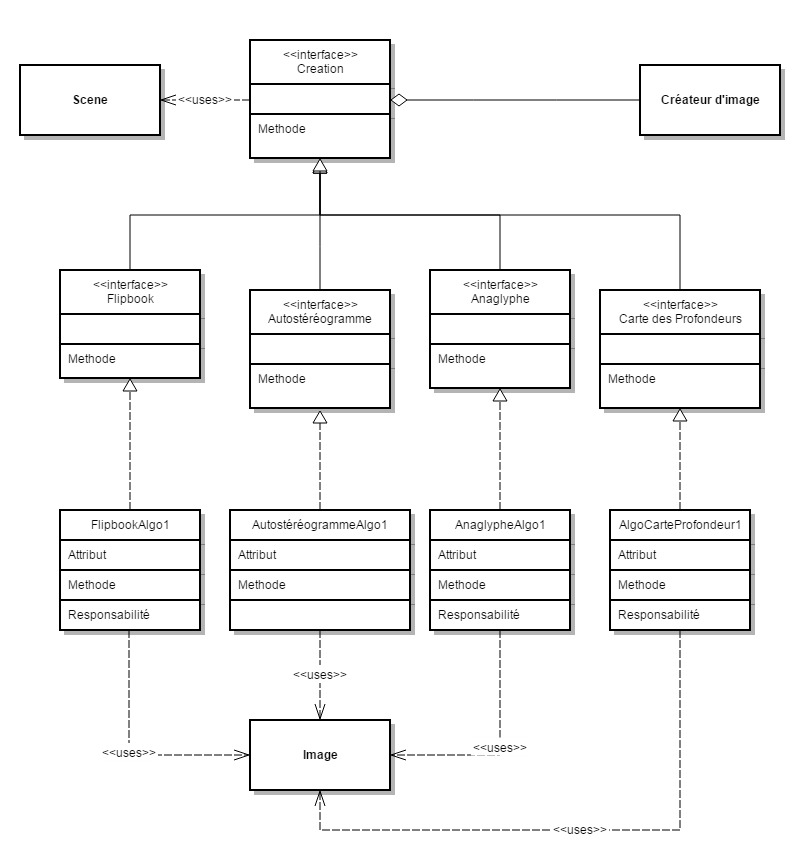
\includegraphics[scale=0.45]{package_creation.jpg}
	\caption{\label{fig:creation} Diagramme des paquetages, architecture globale de la scène \protect \footnotemark}
\end{figure}
\footnotetext{Réalisé grâce au logiciel Gliffy : \url{www.gliffy.com}}

        L'extensibilité de cette architecture se traduit principalement par l'utilisation d'interfaces à différents niveaux. Tout d'abord, le Creator, point d'entrée du paquetage, a pour attribut une première interface Creation qui peut devenir n'importe lequel des rendus souhaité par l'utilisateur. Il peut donc aussi bien devenir un anaglyphe qu'un autostéréogramme. Toutefois, pour permettre l'utilisation de divers algorithmes pour réaliser un même rendu, les classes des rendus sont également des interfaces dont héritent les classes réellement instanciables qui correspondent chacune à un algorithme. On aura donc par exemple AnaglyphAlgorithm1 ou encore DepthMapAlgorithm2.
